\section{Introduction}
\label{sec:introduction}
The best way we know of describing the semantics of parametric
polymorphism is \emph{relational parametricity}, whose central result
is Reynolds' abstraction theorem~\cite{reynolds83types}. Its striking
consequences include the well-known ``free theorems'' for polymorphic
types~\cite{wadler89theorems}, non-inhabitation results, and precise
correspondences between System F encodings and algebraic
datatypes~\cite{PittsAM:parpoe}, abstract data types, and, most
recently, higher-order encodings of binder
syntax~\cite{syntaxforfree}.

Relational parametricity is in essence a principle of
\emph{invariance}: the behaviour of polymorphic code is invariant
under changes of data representation. For example, the type
$\forall\alpha.\tyPrim{list}\alpha\to\tyPrim{list}\alpha$
tells us that any transformation applied to elements of
the input list will be reflected by the same transformation applied
to elements of the result. 
Invariance results also abound in
mathematics and physics. The area of a triangle is invariant with
respect to isometries of the Euclidean plane; the determinant of a
matrix is invariant under changes of basis; and Newton's laws are the
same in all inertial frames. Typically, the 
transformations under which invariants are preserved have interesting structure: 
for example, translations in
the Euclidean plane form an abelian group.

Inspired by this connection, we study type systems that
capture rich invariants through types indexed by attributes with
algebraic structure.  For example, in computational geometry, points
in the plane can be indexed by attributes representing affine
transformations; in information-flow security, computations can be
indexed by principals; in differential privacy, types can be indexed
by `distance'. Types that are polymorphic over such indices induce
invariance properties and abstraction barriers beyond those introduced
by their unindexed versions, as we shall illustrate.  This generalises
previous work by the third author on types parameterized by
units-of-measure, whose invariance properties relate to changes of
units, or \emph{scaling}~\cite{kennedy97relational}.

Our motivations for studying algebraically indexed types are
threefold. First, we believe that, as with
units-of-measure~\cite{fsharp}, practical programming language
extensions will follow. For example, in computational geometry and
graphics, attributes on points, vectors, and other geometric types
could be used to prevent the mixing of different coordinate systems,
or `frames'. Second, type-based static analyses can be based on
indexed types, for example, in effect systems~\cite{benton06reading},
and, more speculatively, in continuity
analysis~\cite{chaudhuri10continuity}.  Finally, we believe that
expressing algebraic invariants through types has the potential to
offer slick proof techniques for mechanized
mathematics. Harrison has applied the
invariance properties of geometric primitives to create elegant proofs
in geometry, based on `without loss of
generality' principles~\cite{harrison09without}. The invariance properties are expressed 
and propagated using ad-hoc tactics; our types offer a more principled
means of achieving the same end, and the `wlog' principle itself
is expressed through type isomorphisms.

We follow the mantra \emph{semantics first, syntax later} in studying
types with algebraic structure. We have not yet built a practical
programming language that supports algebraically indexed types; nor
have we designed type checking, type inference, or static analysis
algorithms.  But when we do so, the semantics will guide us. The fact
that zero is polymorphic in units-of-measure (it can be given type $\forall
u.\tyPrim{real}u$) whereas other constants are dimensionless (having
type $\tyPrim{real}1$) is justified by the invariance properties
induced by the types: zero is invariant under scaling, other constants
are not. For less trivial constants and operations, the appropriate types are
not so apparent, as we shall see, but invariance properties expressed by
the semantics guide us in assigning appropriate types. Semantics does not lie!


\paragraph{Invariance}
To illustrate type-induced invariance properties, consider
2-dimensional geometry. 
A function $\mathit{areaTri}$ that computes the area of a triangle
can be assigned the type:
$\tyPrimNm{vec}\times\tyPrimNm{vec}\times\tyPrimNm{vec}\tyArr\tyReal$.
But we can also assign it the following more expressive polymorphic
type:
\[
\mathrm{areaTri} : \forall t\mathord:\SynTransl{2}.
  \tyPrim{vec}{t} \times \tyPrim{vec}{t} \times \tyPrim{vec}{t} \to \tyReal \\
\]
This type expresses the fact that if each of the arguments to $\mathrm{areaTri}$
is translated by the same vector, then the result remains the same,
that is, it is \emph{invariant} under translation. Formally, for any 
vector $\vec t$,
\[
\mathrm{areaTri}\;(\vec{t} + \vec{v_1}, \vec{t} + \vec{v_2}, \vec{t} + \vec{v_3}) = 
\mathrm{areaTri}\;(\vec{v_1}, \vec{v_2}, \vec{v_3})
\]

Transformations typically \emph{compose} in various
ways, and the compositions satisfy algebraic laws. For example, 
we can assign a function that computes the area of a circle given its
radius the following polymorphic type:
\[
\mathrm{areaCircle} : \forall s\mathord:\SynGL{1}.\tyPrim{real}{s}\to
\tyPrim{real}{s\cdot s}
\]
This captures the fact that the area of a circle varies as the square
of its radius, i.e., $\mathrm{areaCircle}(k r) = k^2\cdot
\mathrm{areaCircle}(r)$ for any $k\neq 0$ (the `sorts' $\SynTransl{2}$ and
$\SynGL{1}$ will be explained later).  Here, $s$ 
can be interpreted as the \emph{units of measure} of the argument to
$\mathrm{areaCircle}$, and `$\cdot$' composes units using the
product. We can also add an inverse operation and identity unit of
measure $1$, and then impose the algebraic laws of abelian
groups. This permits identification of, for example,
$\tyPrim{real}{s\cdot s^{-1}}$ with the type
$\tyPrim{real}{1}$ of dimensionless constants.

\paragraph{Abstraction}
In his original paper on parametricity, Reynolds asserted that
\emph{type structure is a syntactic discipline for enforcing levels of
  abstraction}.  We see something analogous here: if all primitive
operations are given types that reflect their behaviour under
translation, then there is no way to `break' this property. For
example, there is no way that $\mathrm{areaTri}$ can depend on the
actual coordinates of its inputs. Furthermore, the distinction between
points and vectors that is often enforced through abstract data
types~\cite{CGAL} is captured here by indices instead. For example,
the operation that takes two points and computes their vector
difference can be assigned the type
$\forall t\mathord:\SynTransl{2}.\tyPrim{vec}t\times\tyPrim{vec}t\to\tyPrim{vec}0$,
reflecting the invariance of the result (a pure vector) under
translations of the point arguments. As a result through types alone
we can, in essence, derive so-called \emph{coordinate-free}
geometry~\cite{CFGADT}.

The invariance properties discussed above can be seen as ``free
theorems''~\cite{wadler89theorems}, but the abstraction afforded by
polymorphic indexed types can also induce interesting type
\emph{isomorphisms}.  The type of $\mathrm{areaCircle}$ above is in
fact isomorphic to $\tyPrim{real}{1}$. A moment's thought reveals why:
what possible unary functions can be constructed whose outputs scale
as the square of the scaling of their inputs?  Answer: just those
functions of the form~$\lambda x. k x^2$ for some constant~$k$.  In
this case, of course, we expect that~$k = \pi$.

\paragraph{Relational parametricity}
To derive such invariance and abstraction properties of types, we
adopt the techniques of relational parametricity. Over an underlying
index-erasure semantics we construct binary relations parameterised by
an environment $\rho$ that describes how values of primitive type are
related according to their indices.  For example, values $v$ and $w$
of type $\tyPrim{real}s$ are related when $v$ ``scales to'' $w$
according to an interpretation of $s$ (i.e., $w=\rho(s)\cdot
v$).  Values of polymorphic type are related exactly when they are
related for all possible interpretations of the quantified
variable. For example, values $v$ and $w$ of type
$\forall t\mathord:\SynTransl{2}.\tyPrim{vec} t\to
\tyPrim{vec} t$ are related when they are related at type
$\tyPrim{vec} t\to\tyPrim{vec}t$ for all translations
$\vec t\in\Transl{2}$ associated with $t$.

As it happens, the relational interpretations given above are
functional, relating one value uniquely to another. Other applications
make use of primitive relations that are not simple functions.
For example, in a type system in which the index in
$\tyPrim{real}s$ is interpreted not as a unit of measure, but as
a measure of \emph{closeness}, two values $x$ and $y$ of this type are
related if $|x-y| < \rho(s)$ for a positive real number
$\rho(s)$.  Rather beautifully, the standard notion of uniform
continuity can then be expressed as %a type:
%\begin{displaymath}
 $ \forall \epsilon \mathord: \mathsf{R}^{>0}.\ \exists \delta\mathord: \mathsf{R}^{>0}.\ \tyPrim{real}{\delta} \to \tyPrim{real}{\epsilon}$.
%\end{displaymath}


% Possible angles of attack:
% \begin{itemize}
% \item Parametric polymorphic types allow us to prevent
%   over-specification of the behaviour of programs. For instance, the
%   type $\forall \alpha. [\alpha] \to [\alpha]$ is a generalisation of
%   the types $[\mathsf{int}] \to [\mathsf{int}]$ and $[\mathsf{char}]
%   \to [\mathsf{char}]$. Either of the latter two types over-specify
%   the behaviour of the function.
% \item There are other cases of programs that are over-specified. The
%   leading example we just below is of geometric programs that
%   manipulate coordinate data. Often, programs that manipulate
%   coordinate data are insensitive to geometric transformations. For
%   example, a program that computes the area of a triangle described by
%   three points is insensitive to translations or rotations applied to
%   all three points.
% \item 
% \end{itemize}

% There are three main points to get across:
% \begin{enumerate}
% \item Why algebraically indexed types?
% \item Why relational parametricity?
% \item Why study them together?
% \end{enumerate}

\subsection{Contributions}
\label{sec:contributions}

\begin{figure}
  \centering
  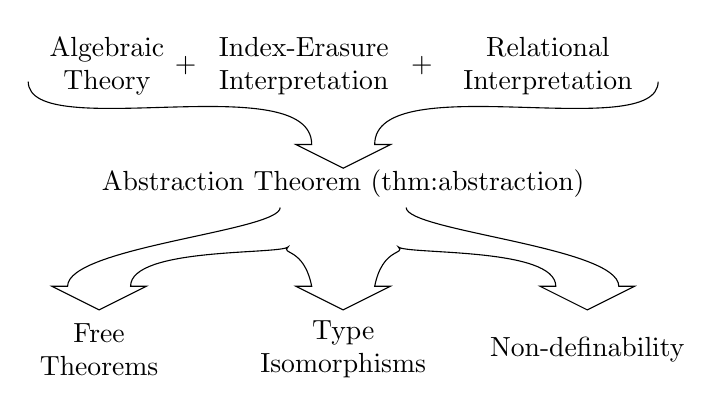
\begin{tikzpicture}
  \node at (-3,0.8) [rectangle,style={align=center}] {Algebraic \\ Theory};
  \node at (-2,0.8) {$+$};
  \node at (-0.5,0.8) [rectangle,style={align=center}] {Index-Erasure \\ Interpretation};
  \node at (1,0.8) {$+$};
  \node at (2.6,0.8) [rectangle,style={align=center}] {Relational \\ Interpretation};
  
  \draw plot (-4,0.6) .. controls (-4,-0.2) and (-0.4,0.8) .. (-0.4,-0.2)
             -- (-0.6,-0.2) -- (0,-0.5) -- (0.6,-0.2) --
             (0.4,-0.2) .. controls (0.4,0.8) and (4,-0.2) .. (4,0.6);

  \node at (0,-0.7) [rectangle,style={align=center}] {Abstraction Theorem (\thmref{thm:abstraction})};

  \draw plot (-0.8,-1) .. controls (-0.8,-1.3) and (-3.5,-1.5) .. (-3.5,-2)
             -- (-3.7,-2) -- (-3.1,-2.3) -- (-2.5,-2) -- 
             (-2.7,-2) .. controls (-2.7,-1.5) and (-0.8,-1.6) .. (-0.7,-1.5)
                       .. controls (-0.8,-1.6) and (-0.5,-1.5) ..
             (-0.4,-2) -- (-0.6,-2) -- (0,-2.3) -- (0.6,-2) --
             (0.4,-2) .. controls (0.5,-1.5) and (0.8,-1.6) .. (0.7,-1.5)
                      .. controls (0.8,-1.6) and (2.7,-1.5) ..
             (2.7,-2) -- (2.5,-2) -- (3.1,-2.3) -- (3.7,-2) -- (3.5,-2)
                      .. controls (3.5,-1.5) and (0.8,-1.3) .. (0.8,-1);

  \node at (-3.1,-2.8) [rectangle,style={align=center}] {Free \\ Theorems};
  \node at (0,-2.8) [rectangle,style={align=center}] {Type \\ Isomorphisms};
  \node at (3.1,-2.8) [rectangle,style={align=center}] {Non-definability};
\end{tikzpicture}
  \caption{Summary of the Paper}
  \label{fig:summary}
\end{figure}

This paper makes the following specific contributions:
\begin{itemize}
\item 
We present a collection of compelling examples of algebraically
indexed types, including a novel type system for geometry, a
refined type system for information flow based on logic, and a simple
type system with distance-indexed types.
\item 
We formulate a type system that can either be used as a programming
language in its own right, or as the target of type-based
analyses. The type system consists of the usual type constructors
together with a collection of indexed primitive types, universal and
existential quantification over the indices, and a multi-sorted
equational theory for indices.
\item
We describe a relational semantics for the type system and prove an
analogue of Reynolds' abstraction theorem, for a given \emph{model}
of index sorts and relational interpretation of primitive types.
We prove that the semantics soundly approximates contextual equivalence.
\item
For each of our main examples we deduce free theorems that are
consequences of our abstraction theorem, prove non-definability
results, and derive interesting type isomorphisms. \autoref{fig:summary}
illustrates the central position of our analogue of Reynolds' Abstraction
Theorem in these results.
\item
We improve on the earlier semantics of
units-of-measure~\cite{kennedy97relational} in a number of ways.  By
extending the language of units with an `absolute value' operation, we
can give more precise types and obtain more general invariance
properties.  The relational interpretation for units is both simpler
and more flexible, and we derive slicker proofs of non-definability,
and new results.  Our notion of type isomorphism is stronger than
previously, being based on contextual equivalence.
\end{itemize}
We have fully formalised our framework and most examples in Coq,
using strongly-typed term representations
throughout~\cite{TypedSyntax}. The formalisation is available from
\\{\small \url{https://github.com/bobatkey/algebraically-indexed-types}}



%%% Local Variables:
%%% TeX-master: "paper"
%%% End:
